\documentclass[thesis=M,english]{FITthesis}[2012/10/20]

% graphics files inclusion
\usepackage{graphicx}
% subfigures
\usepackage{subfig}
% advanced maths
\usepackage{amsmath}
% additional math symbols
\usepackage{amssymb}
% directory tree visualisation
\usepackage{dirtree}

\department{Department of Applied Mathematics}
\title{Neural Networks Based Domain Adaptation in Spectroscopic Sky Surveys}
\authorGN{Ondřej}
\authorFN{Podsztavek}
% author's name without academic degrees
\author{Ondřej Podsztavek}
\authorWithDegrees{Bc. Ondřej Podsztavek}
\supervisor{Petr Škoda}
% TODO acknowledgements
\acknowledgements{}
% TODO english abstract
\abstractEN{}
% TODO czech abstract
\abstractCS{}
\placeForDeclarationOfAuthenticity{Prague}
% TODO english keywords
\keywordsEN{domain adaptation, neural networks, astronomy, spectroscopy}
% TODO czech keywords
\keywordsCS{}
% select according to the desired license (integer 1-6)
\declarationOfAuthenticityOption{2}
% TODO optional thesis URL
%\website{}

\begin{document}

\chapter{Introduction}

How to use neural network based domain adaptation to extract knowledge from the source domain of astronomical spectral data
and apply it to the target astronomical spectral data?

In this work, we would like to prove that astronomical spectroscopy can benefit from domain adapatation (DA).
Previous research has shown that DA can overcome the problem of analysis data from different distribution in one experiment.
In the first chapter~\ref{da_chapter}, we provide a summary of theory of DA, neural networks in DA and DA in astronomy.
Then, in chapter~\ref{data_chapter}, we describe current spectroscopic sky surveys
which might be source of suitable astronomical spectral data.
In experiments~\ref{exp_chapter}, we try to show the benefits of neural DA in astronomy.
Consider that our work is limited to astronomical spectroscopy and neural models.
Having said that, we will apply these methods\dots{}

\section{Problem Definition and Motivation}

The goal of this thesis is the analysis of the impact of domain adaptation in astronomical archives with a focus on neural networks
that would allow using labelled data from one ground-based telescope or space mission archive to discover knowledge in another archive.
Current astronomy has been the primary customer of scalable Big data handling and analysis requirements due to its petabyte-scale archives,
where an advanced machine learning is an indispensable part of workflows leading to new discoveries.

\chapter{Domain Adaptation (DA)}
\label{da_chapter}

Survey the current state of domain adaptation using neural network models in machine learning and with a focus on astronomical applications.

\section{DA in Context of Machine and Transfer Learning}

Now, we introduce the crucial concept of our work: domain adaptation.
Domain adaptation is a subfield of transfer learning,
which is part of machine learning.
Transfer learning is defined in most papers regarding the survey by Pan and Yang~\cite{pan2010}.
A more recent survey by Weiss, Khoshgoftaar and Wang~\cite{weiss2016} has the benefit
that it contains newer methods than the survey by Pan and Yang~\cite{pan2010},
but its definition of transfer learning and domain adaptation is the same.

Machine learning has a common assumption that training and test data are independent and identically distributed
that means samples are drawn from the same feature space and the same distribution.~\cite{daume2006}
When this assumption does not hold transfer learning and domain adaptation come into play.
Moreover, there is a biological inspiration
because humans seem to have natural ways to transfer knowledge from previous experience to new challenges.~\cite{torrey2010}

Pan and Yang define transfer learning as the ability of a system to recognise and apply knowledge and skill learned in previous tasks to novel tasks
and they introduce the notion of a domain and a task.
A domain consists of two components: a feature space and a marginal probability distribution.
Given a specific domain, a task consists of two components: a label space and an objective predictive function
which is not observed but learned from training data.
When we are given a transfer learning problem,
we have to identify a source domain and a source learning task,
a target domain and a target learning task.
Then, transfer learning aims to help improve the learning of the target predictive function in the target domain using knowledge in the source domain and the source task,
where the domains are different or the tasks are different.~\cite{pan2010}

Lastly, Torrey and Shavlik warn that both the source and target domains and tasks need to be sufficiently related
else negative transfer may occur.
Negative transfer is the situation in which the usage of source data degrades the performance.
On the other side, when the performance is improved,
we talk about a positive transfer.~\cite{torrey2010}

\section{Theory and Formalization of DA}

Domain adaptation is the scenario when the source and target domains have different marginal probability distributions
(for example two different telescopes observed the spectra)
while the tasks are the same
(we would like to classify them into the same classes).

\section{Neural Networks in DA}

\section{Previous Applications of DA in Astronomy}

As we have shown, domain adaptation is of great interest to astronomers
because of different instruments, measurements and observation distribution.
Therefore, we survey the current state of domain adaptation in astronomical applications in this section.

If we have a common set of observed stars in both archives,
then we can map them and learn a transfer function.
Ho et al.~\cite{ho2017} did exactly that
% TODO add APOGEE to acronyms
because they found a common set of 9952 spectra in both APOGEE and LAMOST archive.
Using that set, they trained the Cannon method~\cite{ness2015},
and they used the model to transfer some physical parameters from APOGEE to LAMOST.

In the case, when there is no common set Gupta et al. experimented with subspace alignment~\cite{fernando2014} and kernel mean matching~\cite{gretton2009} followed by active learning.~\cite{gupta2016}
In the case of subspace alignment, the negative transfer occurred while the kernel mean matching seems very promising in the task of supernova classification.
Then, Vilalta et al.~\cite{vilalta2018} extended the work of Gupta et al.~\cite{gupta2016}.
Vilalta et al. used a maximum a posteriori (MAP) approach to learn a prior on the model parameters from a spectroscopic source domain
and then use this prior distribution to learn a model in a photometric target domain.
Concretely, Vilalta et al. put a prior on the number of layers of a neural network
and then used active learning.
Richards et al.~\cite{richards2011} faced a similar situation, as Gupta et al.
Richards et al. introduce the problem as sample selection bias~\cite{shimodaira2000} or covariate shift~\cite{heckman1979}
when different distributions generate the source and target data.
That is precisely the problem we have defined as domain adaptation.
Richards et al. experimented with random forest in combination with three domain adaptation methods:
importance weighting~\cite{shimodaira2000}, co-training~\cite{blum1998} and active learning~\cite{settles2009}.
The result is not surprising from our point of view.
Active learning works best while importance weighting and co-training achieve negative transfer.

The term transfer learning has been recently used in the context of deep learning.
However, transfer learning in the context of deep learning means something more concrete than what we defined as transfer learning previously.
Transfer learning in the context of deep learning is the specific situation
when a pretrained deep neural network model is taken,
and its last layers are retrained with the target domain data.
Ackermann et al.~\cite{ackermann2018} employed with the transfer learning approach in the context of deep learning to detect galaxy merges.
Ackermann et al. took the Xception convolutional neural network~\cite{chollet2017}
and retrain its last layers with images of galaxy merger labelled in a citizen science Galaxy Zoo project.
This transfer learning approach allowed Ackermann et al. to lower the best error rate so far by 15\%.

\chapter{Spectroscopic Sky Surveys}
\label{data_chapter}

% TODO chapter summary

Select suitable dataset of astronomical spectra for experiments.

To understand this work we need first to introduce the spectral
data because we are interested in classifying them.

\section{Astronomical Spectroscopy}

Telescopes are giant eyes that can collect much more light that human's eye.
Spectrographs can disperse the light collected by a telescope into spectra
which reveal objects composition, speed, temperature and more.

% TODO cite Bennett (2005) and ESA's webpage about Gaia spectroscopy:
% https://www.esa.int/Science_Exploration/Space_Science/Gaia/Spectroscopy

The visible light is only a tiny part of the complete spectrum of electromagnetic radiation.
The complete spectrum of electromagnetic radiation is usually called the electromagnetic spectrum.
Electromagnetic radiation carries information about stars and planets made of matter across the universe.
The energy carried by light interacts with matter in following ways:

\begin{itemize}
	\item \textit{emission} (an electric current flowing through the bulb heats it to a point at
		which its matter emits visible light);
	\item \textit{absorption} (hand placed near a lit light bulb absorbs some of the light).
\end{itemize}

Spectra come in three basic types, and real astronomical spectra are usually a combination of these types:

\begin{itemize}
	\item the spectrum of a conventional light bulb is a continuous rainbow (called thermal radiation spectrum);
	\item if a cloud of gas lies between a detector and a bulb,
		the cloud can absorb specific wavelength making what an absorption line spectrum;
	\item the cloud might emit light itself; therefore, this spectrum is called an emission-line spectrum.
\end{itemize}

The fact that each atom, ion or molecule possesses a unique set of energy levels
causes emission and absorption lines at specific wavelengths in spectra.
Spectral lines correspond to the wavelengths of light absorbed by chemicals on the surface of the star.
Therefore, positions of emission and absorption lines can tell us objects composition.
We display spectra as bands of light that is a projection of light that passes through a prism on a wall
(see Fig.~\ref{solar_spectrum}).
A more reasonable way is to display spectra as graphs of intensities of the light in each wavelength.

\begin{figure}
	% TODO give credit https://solarsystem.nasa.gov/resources/390/the-solar-spectrum/
	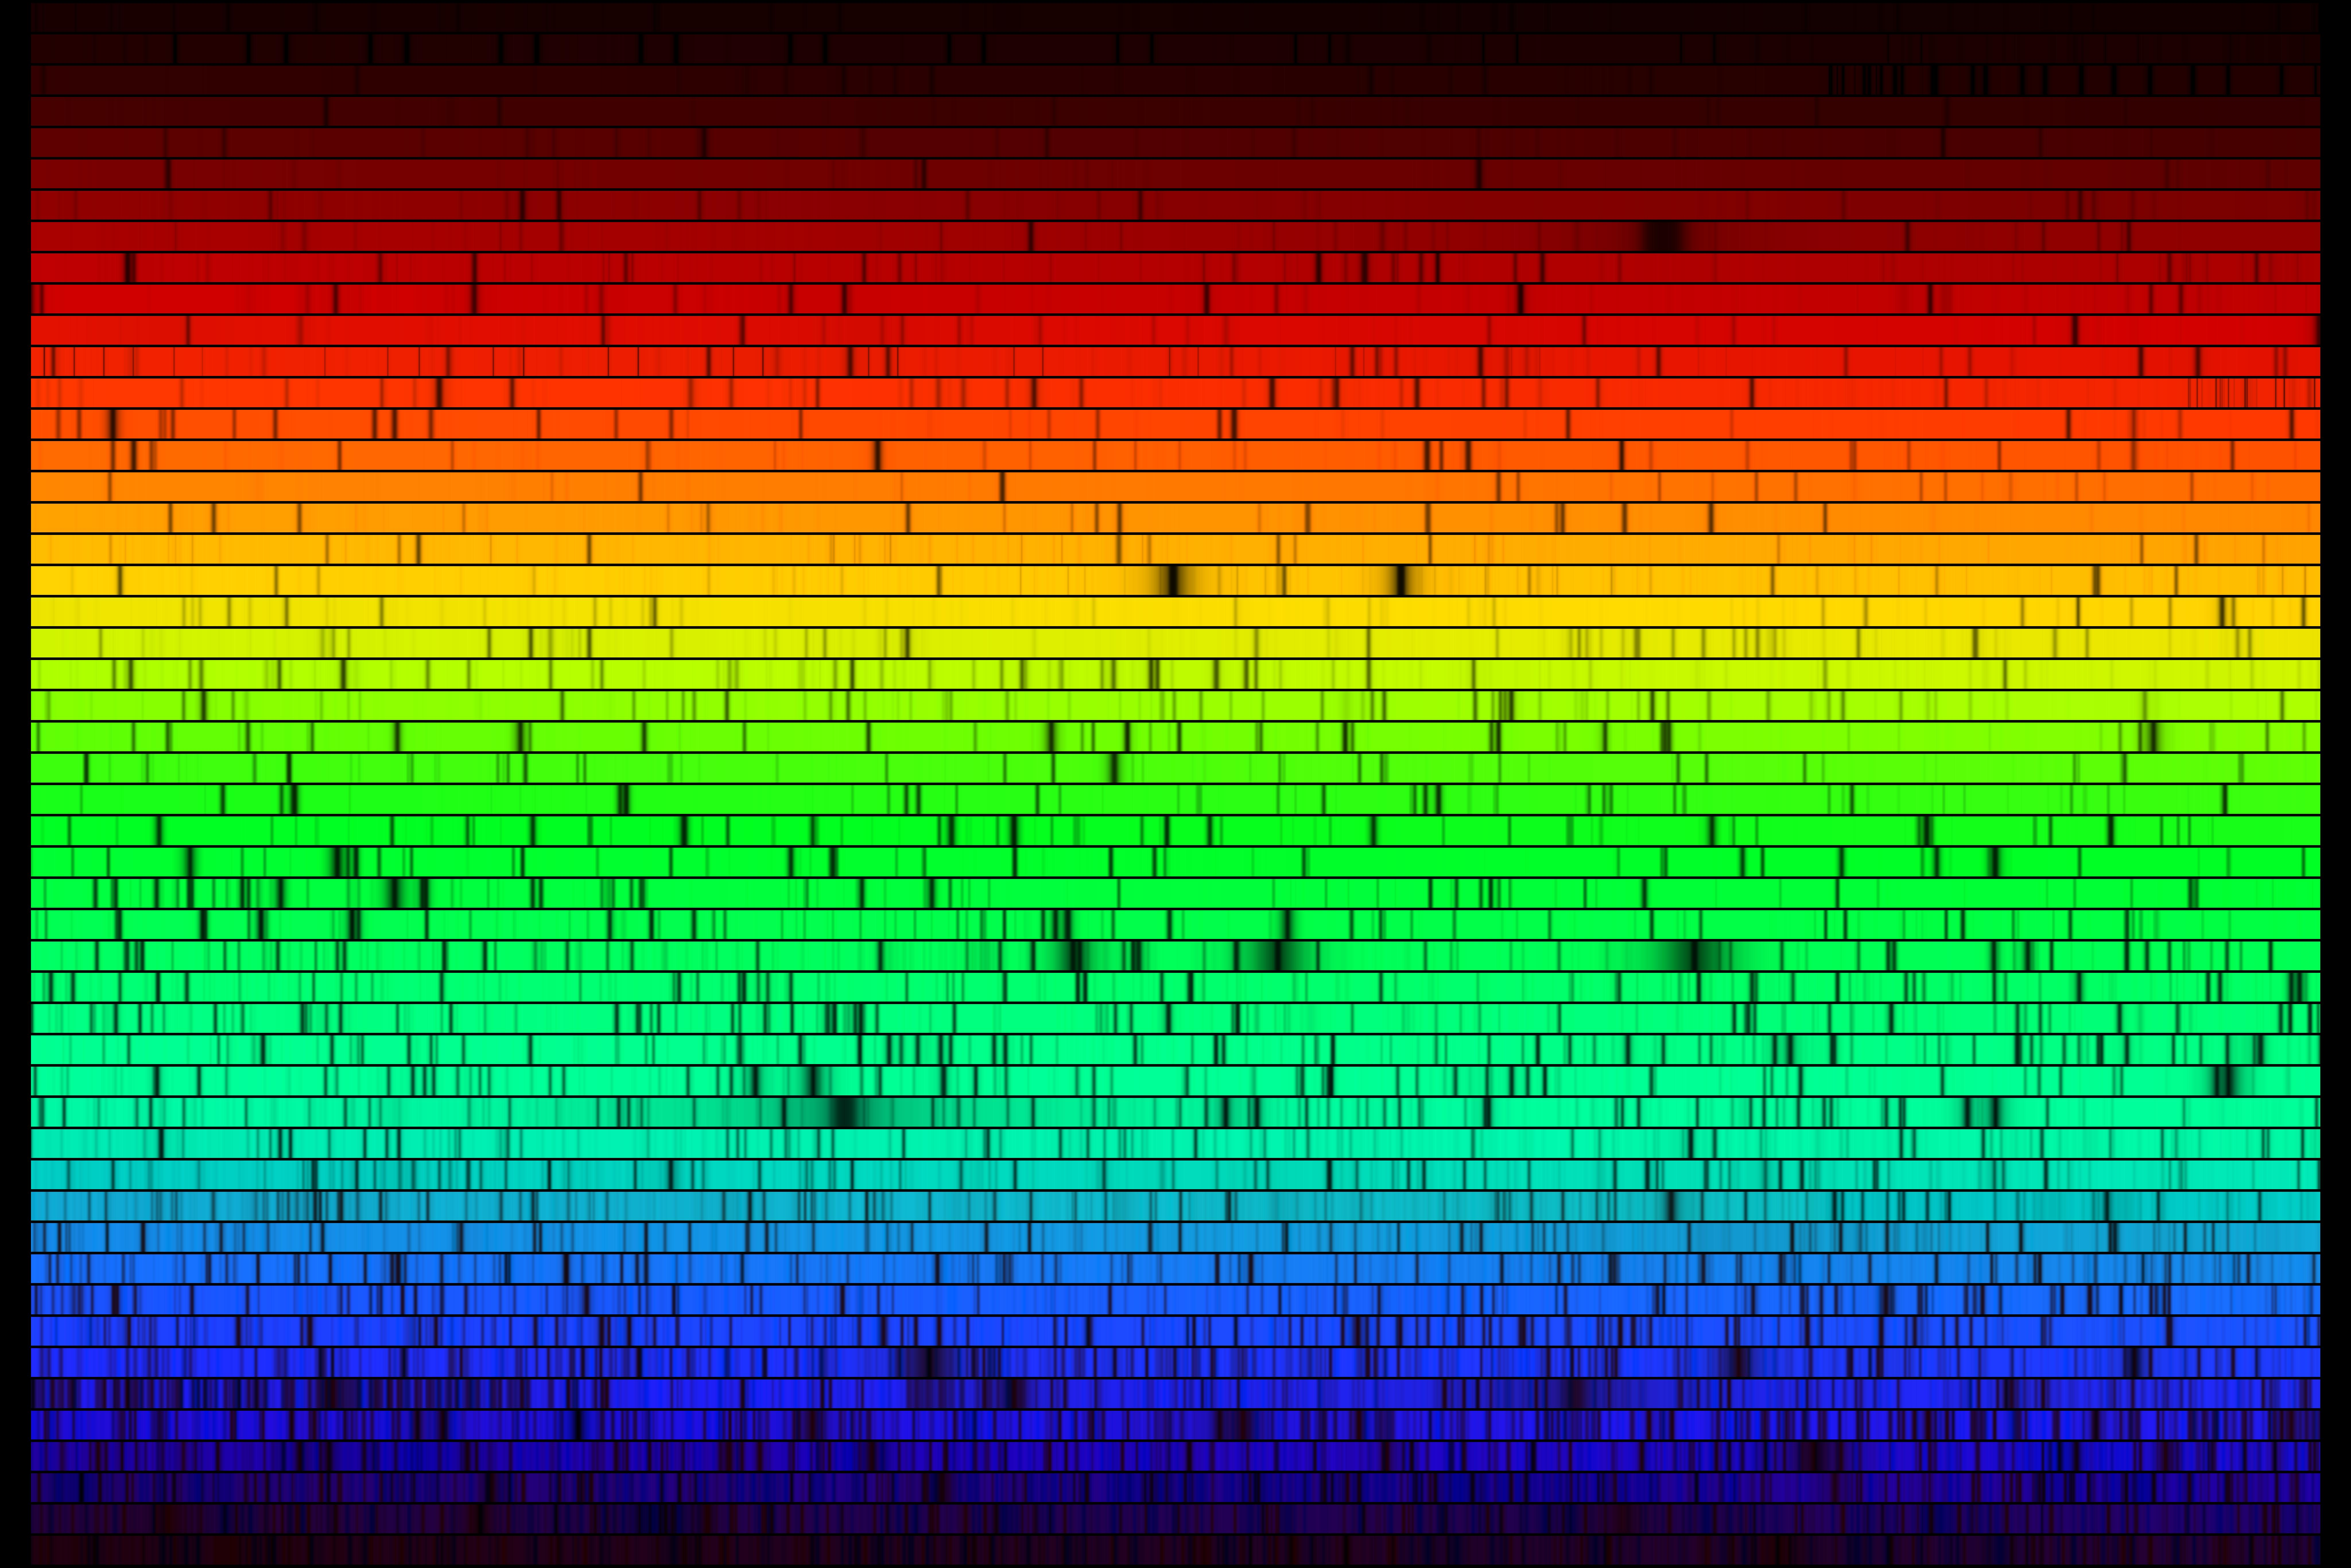
\includegraphics[width=\textwidth]{img/solarspectrum.jpg}
	\caption{The Solar Spectrum (Image by \href{https://solarsystem.nasa.gov/resources/390/the-solar-spectrum/}{NASA})}
	\label{solar_spectrum}
\end{figure}

Finally, we can view an astronomical spectrum as a one-dimensional image.
Therefore, convolutional neural networks seem to be a great tool to analyse them.

\section{Large Spectral Archives}

Give list of large spectral archives focused on observation of QSOs.
Main archives are Ondřejov, LAMOST, Gaia (doesn't have spectra available yet)
and SDSS (similar to LAMOST, optical and IR, APOGEE survey).
Marginal archives are GALEX (ultraviolet), CALIFA or ESO MUSE.

Choose LAMOST and SDSS and tell why we have choosen them.

\subsection{Sloan Digital Sky Survey}

Describe SDSS, its spectra and catalog of QSOs.

\begin{figure}
	% TODO cite https://solarsystem.nasa.gov/resources/390/the-solar-spectrum/
	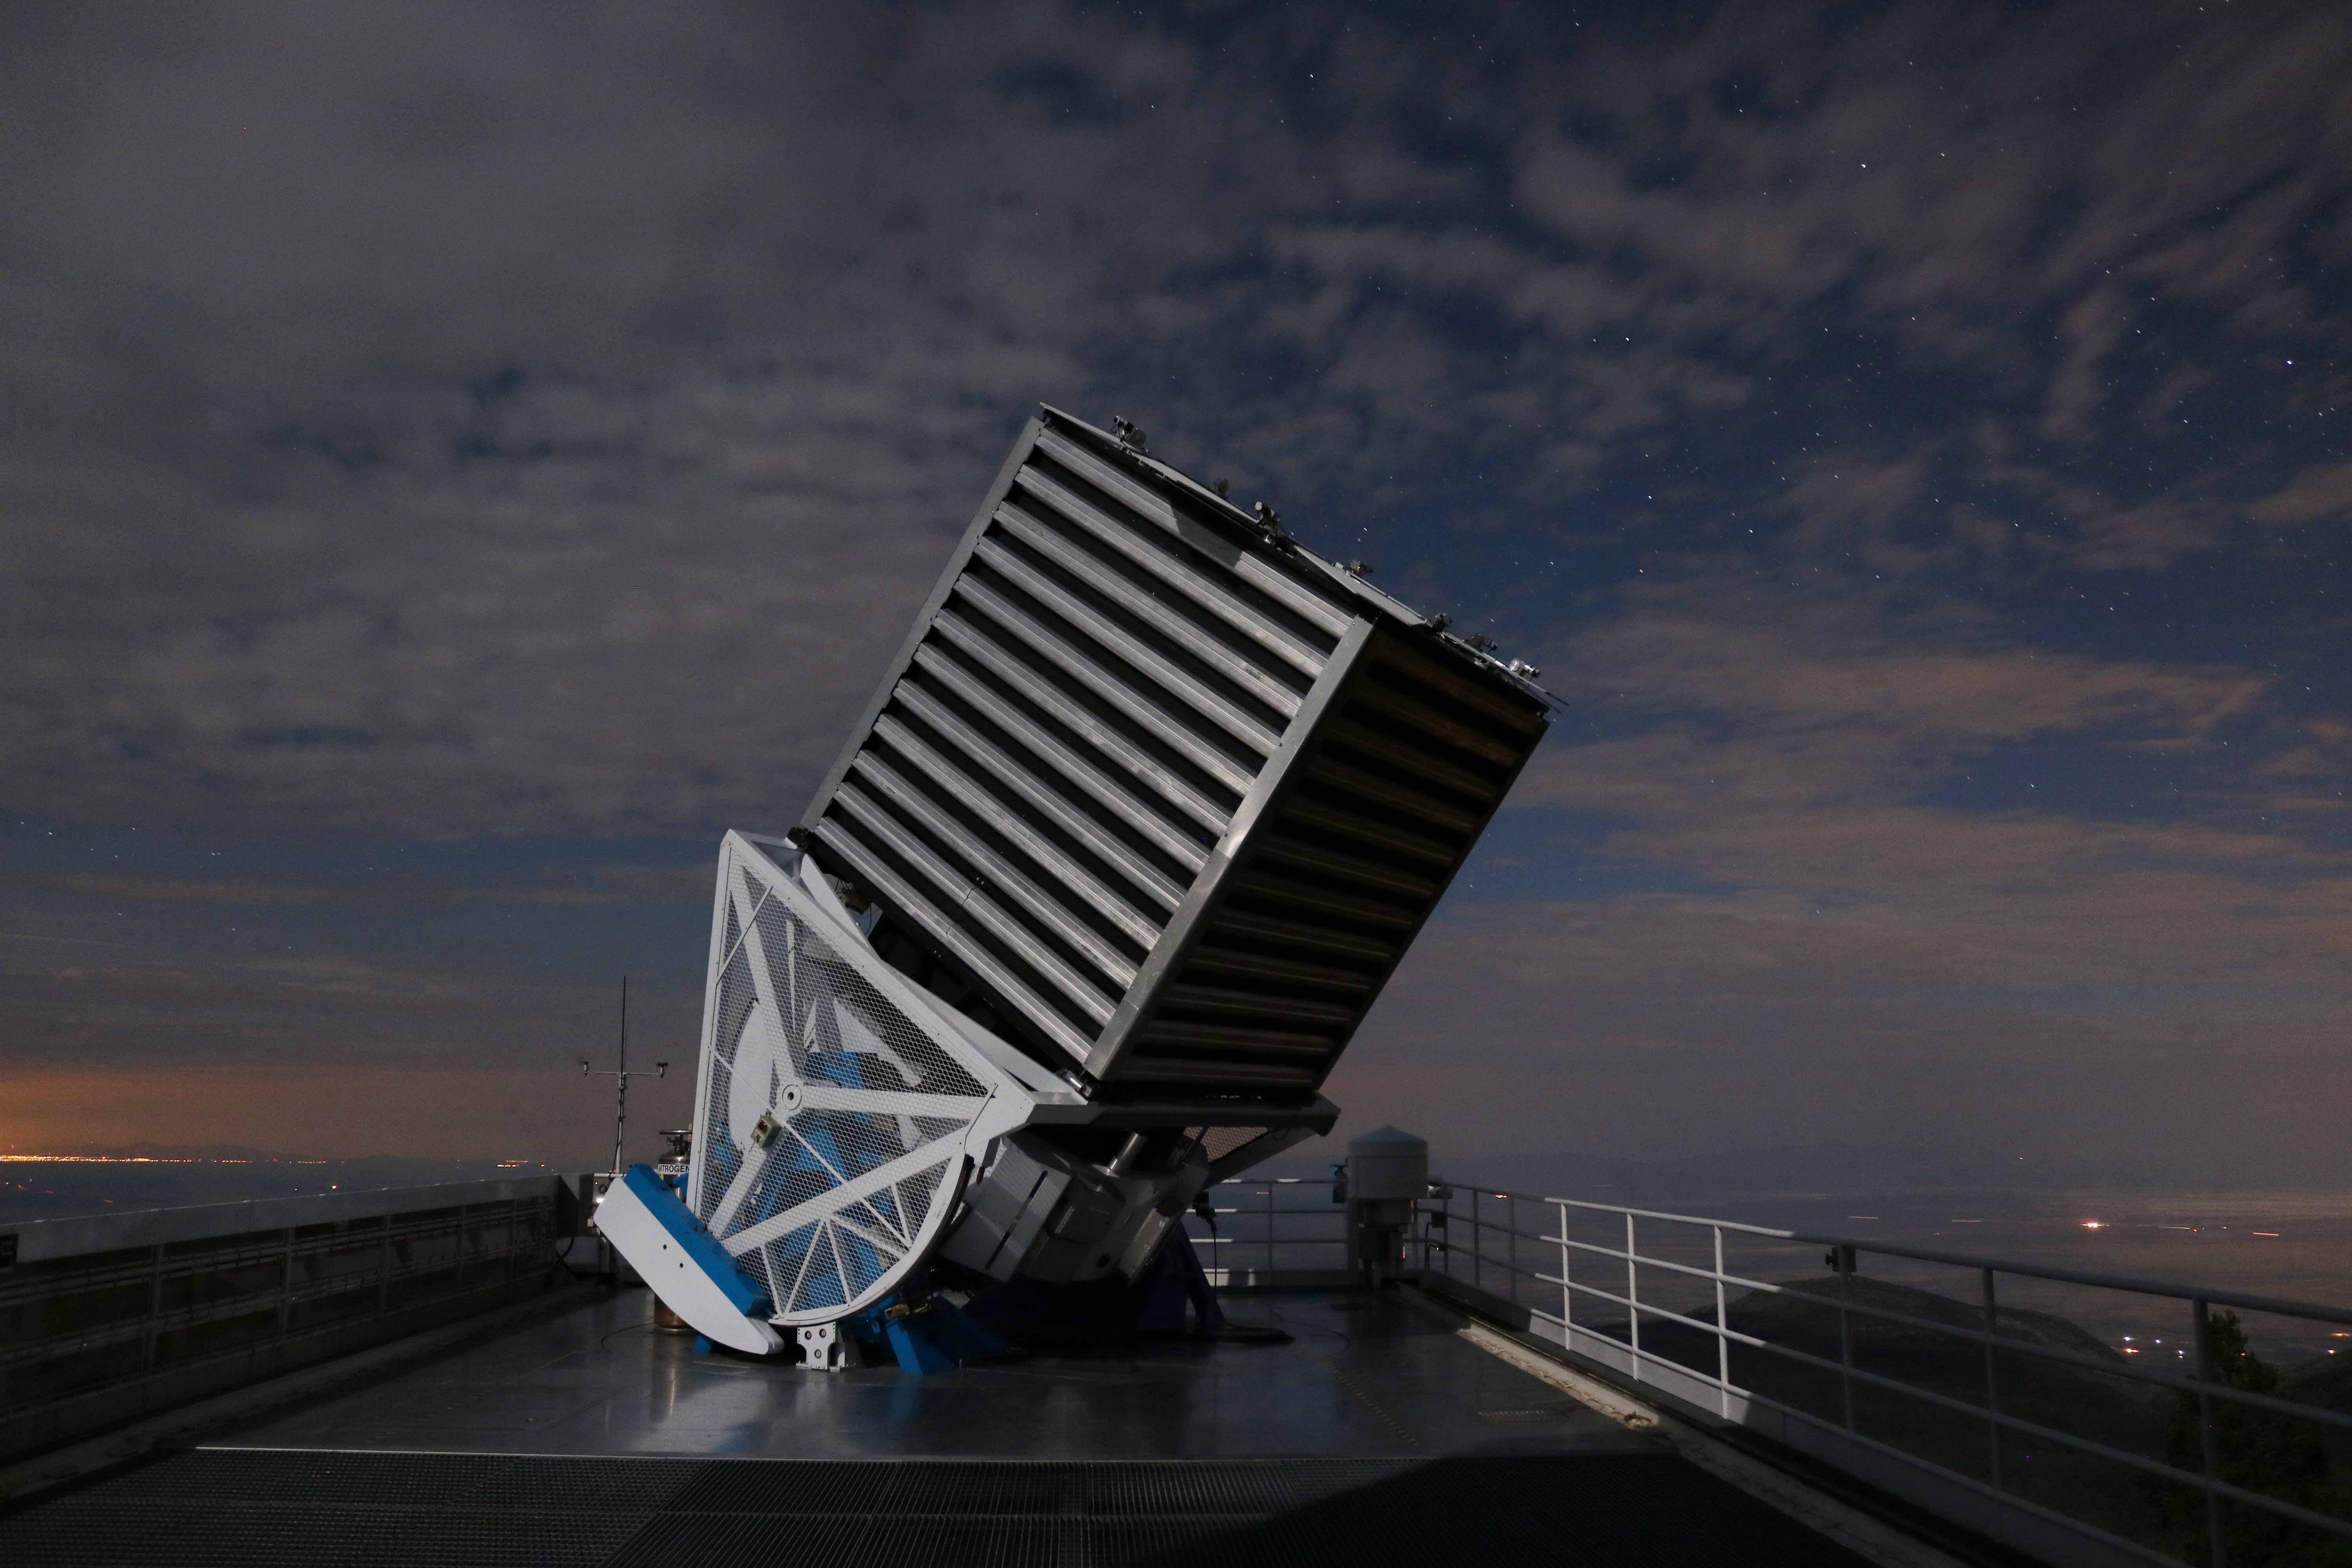
\includegraphics[width=\textwidth]{img/sdss_gaulme.jpg}
	\caption{The SDSS telescope at night (Image by Patrick Gaulme is licensed under CC BY 4.0)}
	\label{solar_spectrum}
\end{figure}

\subsection{Large Sky Area Multi-Object Fiber Spectroscopic Telescope}

Describe LAMOST, its spectra and catalog of QSOs.

\section{Quasi-Stellar Objects}

Also known as \textit{quasars} and abbreviated \textit{QSO}.

\begin{itemize}
	\item Physical definition of QSOs.
	\item Definition of QSOs according SDSS DR14Q.
	\item Why QSOs are interesting? Something as the expanding Universe.
	\item Why QSOs are suitable for experimenting with DA?
		QSOs have big redshift and CNNs are shift invariant.
		Searching for QSOs in different archives.
\end{itemize}

\section{Comparison of the Spectral Data}

Compare instruments, data and sky coverage.

Investigate the structure of data space in selected datasets (dimensionality reduction).

\chapter{Experiments: Application of Neural DA to Spectral Data}
\label{exp_chapter}

\section{Results without use of Neural DA}

\section{Benefits of Neural DA: Analysis and Visualisation of Results}

Apply domain adaptation to the selected data
and prepare visualisation of results.

\chapter{Conclusion}

\section{Discussion of Performance}

Discuss the precision performance and scalability of various solutions.

\section{Future Plans}

Suggest future improvements.

\bibliographystyle{iso690}
\bibliography{references}

\appendix

\chapter{Acronyms}
\begin{description}
    \item[LAMOST] Large Sky Area Multi-Object Fiber Spectroscopis Telescope
\end{description}

\chapter{Contents of Enclosed CD}

\begin{figure}
\dirtree{%
    .1 README.md\DTcomment{the file with CD contents description}.
    .1 src\DTcomment{the directory of source codes}.
    .2 latex\DTcomment{the directory of \LaTeX{} source codes of the thesis}.
    .1 thesis.pdf\DTcomment{the thesis text in PDF format}.
}
\end{figure}

\end{document}
